\documentclass[a4paper,10pt]{article}
\usepackage[brazilian]{babel}
\usepackage[left=2.5cm,right=2.5cm,top=3cm,bottom=2.5cm]{geometry}
\usepackage{mathtools}
\usepackage{amsthm}
\usepackage{amsmath}
%\usepackage{nccmath}
\usepackage{amssymb}
\usepackage{amsfonts}
\usepackage{physics}
%\usepackage{dsfont}
%\usepackage{mathrsfs}

\usepackage{titling}
\usepackage{indentfirst}

\usepackage{bm}
\usepackage[dvipsnames]{xcolor}
\usepackage{cancel}

\usepackage{xurl}
\usepackage[colorlinks=true]{hyperref}

\usepackage{float}
\usepackage{graphicx}
%\usepackage{tikz}
\usepackage{caption}
\usepackage{subcaption}

%%%%%%%%%%%%%%%%%%%%%%%%%%%%%%%%%%%%%%%%%%%%%%%%%%%

\newcommand{\eps}{\epsilon}
\newcommand{\vphi}{\varphi}
\newcommand{\cte}{\text{cte}}

\newcommand{\N}{\mathbb{N}}
\newcommand{\Z}{\mathbb{Z}}
\newcommand{\Q}{\mathbb{Q}}
\newcommand{\R}{\vb{R}}
\newcommand{\C}{\mathbb{C}}
\renewcommand{\S}{\hat{S}}
%\renewcommand{\H}{\s{H}}

\renewcommand{\a}{\vb{a}}
\newcommand{\nn}{\hat{n}}
\renewcommand{\d}{\dagger}
\newcommand{\up}{\uparrow}
\newcommand{\down}{\downarrow}

\newcommand{\0}{\vb{0}}
%\newcommand{\1}{\mathds{1}}
\newcommand{\E}{\vb{E}}
\newcommand{\B}{\vb{B}}
\renewcommand{\v}{\vb{v}}
\renewcommand{\r}{\vb{r}}
\renewcommand{\k}{\vb{k}}
\newcommand{\p}{\vb{p}}
\newcommand{\q}{\vb{q}}
\newcommand{\F}{\vb{F}}

\newcommand{\s}{\sigma}
%\newcommand{\prodint}[2]{\left\langle #1 , #2 \right\rangle}
\newcommand{\cc}[1]{\overline{#1}}
\newcommand{\Eval}[3]{\eval{\left( #1 \right)}_{#2}^{#3}}

\newcommand{\unit}[1]{\; \mathrm{#1}}

\newcommand{\n}{\medskip}
\newcommand{\e}{\quad \mathrm{e} \quad}
\newcommand{\ou}{\quad \mathrm{ou} \quad}
\newcommand{\virg}{\, , \;}
\newcommand{\ptodo}{\forall \,}
\renewcommand{\implies}{\; \Rightarrow \;}
%\newcommand{\eqname}[1]{\tag*{#1}} % Tag equation with name

\setlength{\droptitle}{-7em}

\theoremstyle{plain}
\newtheorem{theorem}{Teorema}[section]
%\newtheorem{defi}[theorem]{Definição}
\newtheorem{lemma}[theorem]{Lema}
%\newtheorem{corol}[theorem]{Corolário}
%\newtheorem{prop}[theorem]{Proposição}
%\newtheorem{example}{Exemplo}
%
%\newtheorem{inneraxiom}{Axioma}
%\newenvironment{axioma}[1]
%  {\renewcommand\theinneraxiom{#1}\inneraxiom}
%  {\endinneraxiom}
%
%\newtheorem{innerpostulado}{Postulado}
%\newenvironment{postulado}[1]
%  {\renewcommand\theinnerpostulado{#1}\innerpostulado}
%  {\endinnerpostulado}
%
%\newtheorem{innerexercise}{Exercício}
%\newenvironment{exercise}[1]
%  {\renewcommand\theinnerexercise{#1}\innerexercise}
%  {\endinnerexercise}
%
%\newtheorem{innerthm}{Teorema}
%\newenvironment{teorema}[1]
%  {\renewcommand\theinnerthm{#1}\innerthm}
%  {\endinnerthm}
%
\newtheorem{innerlema}{Lema}
\newenvironment{lema}[1]
  {\renewcommand\theinnerlema{#1}\innerlema}
  {\endinnerlema}
%
%\theoremstyle{remark}
%\newtheorem*{hint}{Dica}
%\newtheorem*{notation}{Notação}
%\newtheorem*{obs}{Observação}


\title{\Huge{\textbf{Lista 4 - Matéria Condensada 2}}}
\author{Mateus Marques}

\renewcommand{\lg}{\text{lg}}

\begin{document}

\maketitle

\section{Modelo de Hubbard}

(a) Na questão 3 da Lista 1 eu cheguei a calcular $\S_i \vdot \S_j$. Lá eu obtive
$$
\S_i \vdot \S_j = -\frac{1}{2} \sum_{\s, \s'} c_{i\s}^\d c_{j\s'}^\d c_{i\s'} c_{j\s} - \frac{1}{4} n_i n_{j}.
$$

Temos então que para $i=j$:
$$
\S_i^2 = -\frac{1}{2} \sum_{\s,\s'} c_{i\s}^\d n_{i\s'} c_{i\s} - \frac{1}{4} n_i^2.
$$

Usando que $[c_{i\s}^\d, n_{i\s'}] = - \delta_{\s\s'} c_{i\s}^\d$ e $n_i^2 = (n_{i\up} + n_{i\down})^2 = n_i + 2 n_{i\up} n_{\down}$, temos
$$
\S_i^2 = -\frac{1}{2} \sum_{\s,\s'} \qty(n_{i\s'} c_{i\s}^\d - \delta_{\s\s'} c_{i\s}^\d ) c_{i\s} - \frac{1}{4} (n_i + 2 n_{i\up} n_{i\down}) \implies
$$
$$
\S_i^2 = -\frac{1}{2} \sum_{\s,\s'} n_{i\s'} n_{i\s} + \sum_{\s} n_{i\s} - \frac{1}{4} (n_i + 2 n_{i\up} n_{i\down}) \implies
$$
$$
\S_i^2 = -\frac{1}{2} (n_i + 2 n_{i\up} n_{\down}) + n_i - \frac{1}{4} n_i - \frac{1}{2} n_{i\up} n_{i\down} =
\frac{1}{4} n_i - \frac{3}{2} n_{i\up} n_{i\down} \implies
$$
$$
n_{i\up} n_{i\down} = -\frac{2}{3} \S_i^2 + \frac{1}{2} n_i \implies
\boxed{
U \sum_{i} n_{i\up} n_{i\down} =
-\frac{2}{3} \sum_{i} (\S_i^2) + \frac{U}{2} \sum_{i} n_i.
}
$$

Para mostrar que $[H, N_e] = 0$, é óbvio que cada $n_{i\up}$ e $n_{i\down}$ comutam com os termos \textit{interaction} e \textit{on-site} da hamiltoniana. Assim, falta mostrar que $N_e$ comuta com o termo de \textit{hopping}. Note que
$$
[c_{i\s}^\d c_{j\s} + c_{j\s}^\d c_{i\s}, n_{k\s'}] =
\Big([c_{i\s}^\d, n_{k\s'}] c_{j\s} + c_{i\s}^\d [c_{j\s}, n_{k\s'}]\Big) +
\Big([c_{j\s}^\d, n_{k\s'}] c_{i\s} + c_{j\s}^\d [c_{i\s}, n_{k\s'}]\Big)
$$
$$
=
\delta_{\s\s'} \Big(-c_{i\s}^\d c_{j\s} \delta_{ik} + c_{i\s}^\d c_{j\s} \delta_{jk} -
c_{j\s}^\d c_{i\s} \delta_{jk} + c_{j\s}^\d c_{i\s} \delta_{ik} \Big)
$$

Assim, para qualquer spin $\s' = \; \up, \down$, temos
$$
\qty[\sum_{\nn{i}{j}, \s} (c_{i\s}^\d c_{j\s} + c_{j\s}^\d c_{i\s}),
\sum_{k} n_{k\s'} ] =
\delta_{\s\s'} \sum_{\nn{i}{j}, \s}
\qty( \cancelto{0}{\boxed{-c_{i\s}^\d c_{j\s} + c_{i\s}^\d c_{j\s}}} \; \cancelto{0}{\boxed{- c_{j\s}^\d c_{i\s} + c_{j\s}^\d c_{i\s}}} ) = 0.
$$

Como $N_e = \sum_{\s} \sum_{k} n_{k\s}$, vemos que $[H, N_e] = 0$.

\n

Para a magnetização $M^z$, também é óbvio que ela comuta com os termos de \textit{interaction} e \textit{on-site}. Escrevendo $2 M^z = \sum_{k} n_{k\up} - \sum_{k} n_{k\down}$, do resultado anterior é direto que $M^z$ também comuta com o termo de \textit{hopping}. Isso nos dá que $[H, M^z] = 0$.

\pagebreak

(b) As duas sub-redes da rede quadrada são facilmente identificadas, como na Figura \ref{fig:square-lat}:
\begin{figure}[H]
\centering
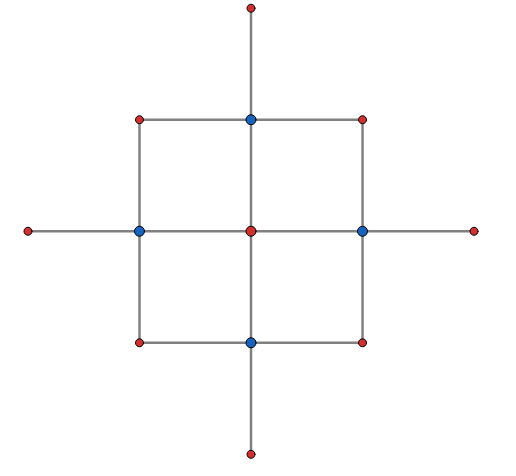
\includegraphics[width=0.4\textwidth]{fig/square-lat.png}
\caption{Rede quadrada e suas sub-redes $\textcolor{red}{A}$ e $\textcolor{blue}{B}$.}
\label{fig:square-lat}
\end{figure}


A transformação partícula-buraco \textbf{na verdade} (c.f. notas de aula) é dada por
$$
c_{i\s} =
\begin{cases}
\; -d_{i\s}^\d, \quad i \in A; \\
\; +d_{i\s}^\d, \quad i \in B.
\end{cases}
$$

Para uma rede bipartida, a parte de \textit{hopping} do hamiltoniano é dado por
$$
H_t = -t \sum_{\s, \R_i, \bm{\delta}} \Big[
c_{\R_i, A, \s}^\d c_{\R_i + \bm{\delta}, B, \s} +
c_{\R_i, B, \s}^\d c_{\R_i + \bm{\delta}, A, \s}
\Big].
$$

Sobre a transformação partícula-buraco, temos que
$$
c_{\R_i, A, \s}^\d c_{\R_i + \bm{\delta}, B, \s} +
c_{\R_i, B, \s}^\d c_{\R_i + \bm{\delta}, A, \s} =
- d_{\R_i, A, \s} d_{\R_i + \bm{\delta}, B, \s}^\d
- d_{\R_i, B, \s} d_{\R_i + \bm{\delta}, A, \s}^\d =
$$
$$
= d_{\R_i, A, \s}^\d d_{\R_i + \bm{\delta}, B, \s} +
d_{\R_i, B, \s}^\d d_{\R_i + \bm{\delta}, A, \s},
$$
ou seja, $H_t$ se mantém invariante sobre a transformação partícula-buraco.

Se definirmos $H_U$ como
$$
H_U = U \sum_{i} (n_{i\up} - 1/2) (n_{i\down} - 1/2),
$$
temos que ele também se mantém invariante. Note que $n_{i\s} = c_{i\s}^\d c_{i\s} = d_{i\s} d_{i\s}^\d = 1 - d_{i\s}^\d d_{i\s}$, logo
$$
(c_{i\up}^\d c_{i\up} - 1/2) (c_{i\down}^\d c_{i\down} - 1/2) =
(1/2 - d_{i\up}^\d d_{i\up}) (1/2 - d_{i\down}^\d d_{i\down}) =
(d_{i\up}^\d d_{i\up} - 1/2) (d_{i\down}^\d d_{i\down} - 1/2).
$$
Assim, $H_U$ também se mantém invariante.

Porém, para a parte $H_{\tilde{\mu}}$, definida como
$$
H_{\tilde{\mu}} =
-\tilde{\mu} \sum_{i} (n_{i\up} + n_{i\down}) =
-\tilde{\mu} \sum_{i} (c_{i\up}^\d c_{i\up} + c_{i\down}^\d c_{i\down}) =
-\tilde{\mu} \sum_{i} (2 - d_{i\up}^\d d_{i\up} - d_{i\down}^\d d_{i\down}),
$$
não se mantém invariante a menos que $\tilde{\mu} = 0$, que é justamente a situação de semipreenchimento $\mu = U/2$, quando todo o hamiltoniano de Hubbard possui simetria partícula-buraco.

\n

(c) No limite atômico $t = 0$, como os sítios são independentes, a função de partição é simplesmente dada por $Z = 1 + 2 e^{\beta \mu} + e^{\beta(2\mu - U)}$. A ocupação média $n$ é dada então por
$$
n = \frac{1}{\beta Z} \cdot \pdv{Z}{\mu} =
\frac{2 e^{\beta\mu} + 2 e^{\beta(2\mu-U)}}{1 + 2 e^{\beta \mu} + e^{\beta(2\mu - U)}}.
$$
\textbf{FAZER O GRÁFICO.}




\pagebreak

\section{Antiferromagnetismo no modelo de Hubbard em campo médio}

(a) A magnetização no espaço real para o estado de Néel na rede quadrada é esboçada na Figura \ref{fig:mag-neel}:
\begin{figure}[H]
\centering
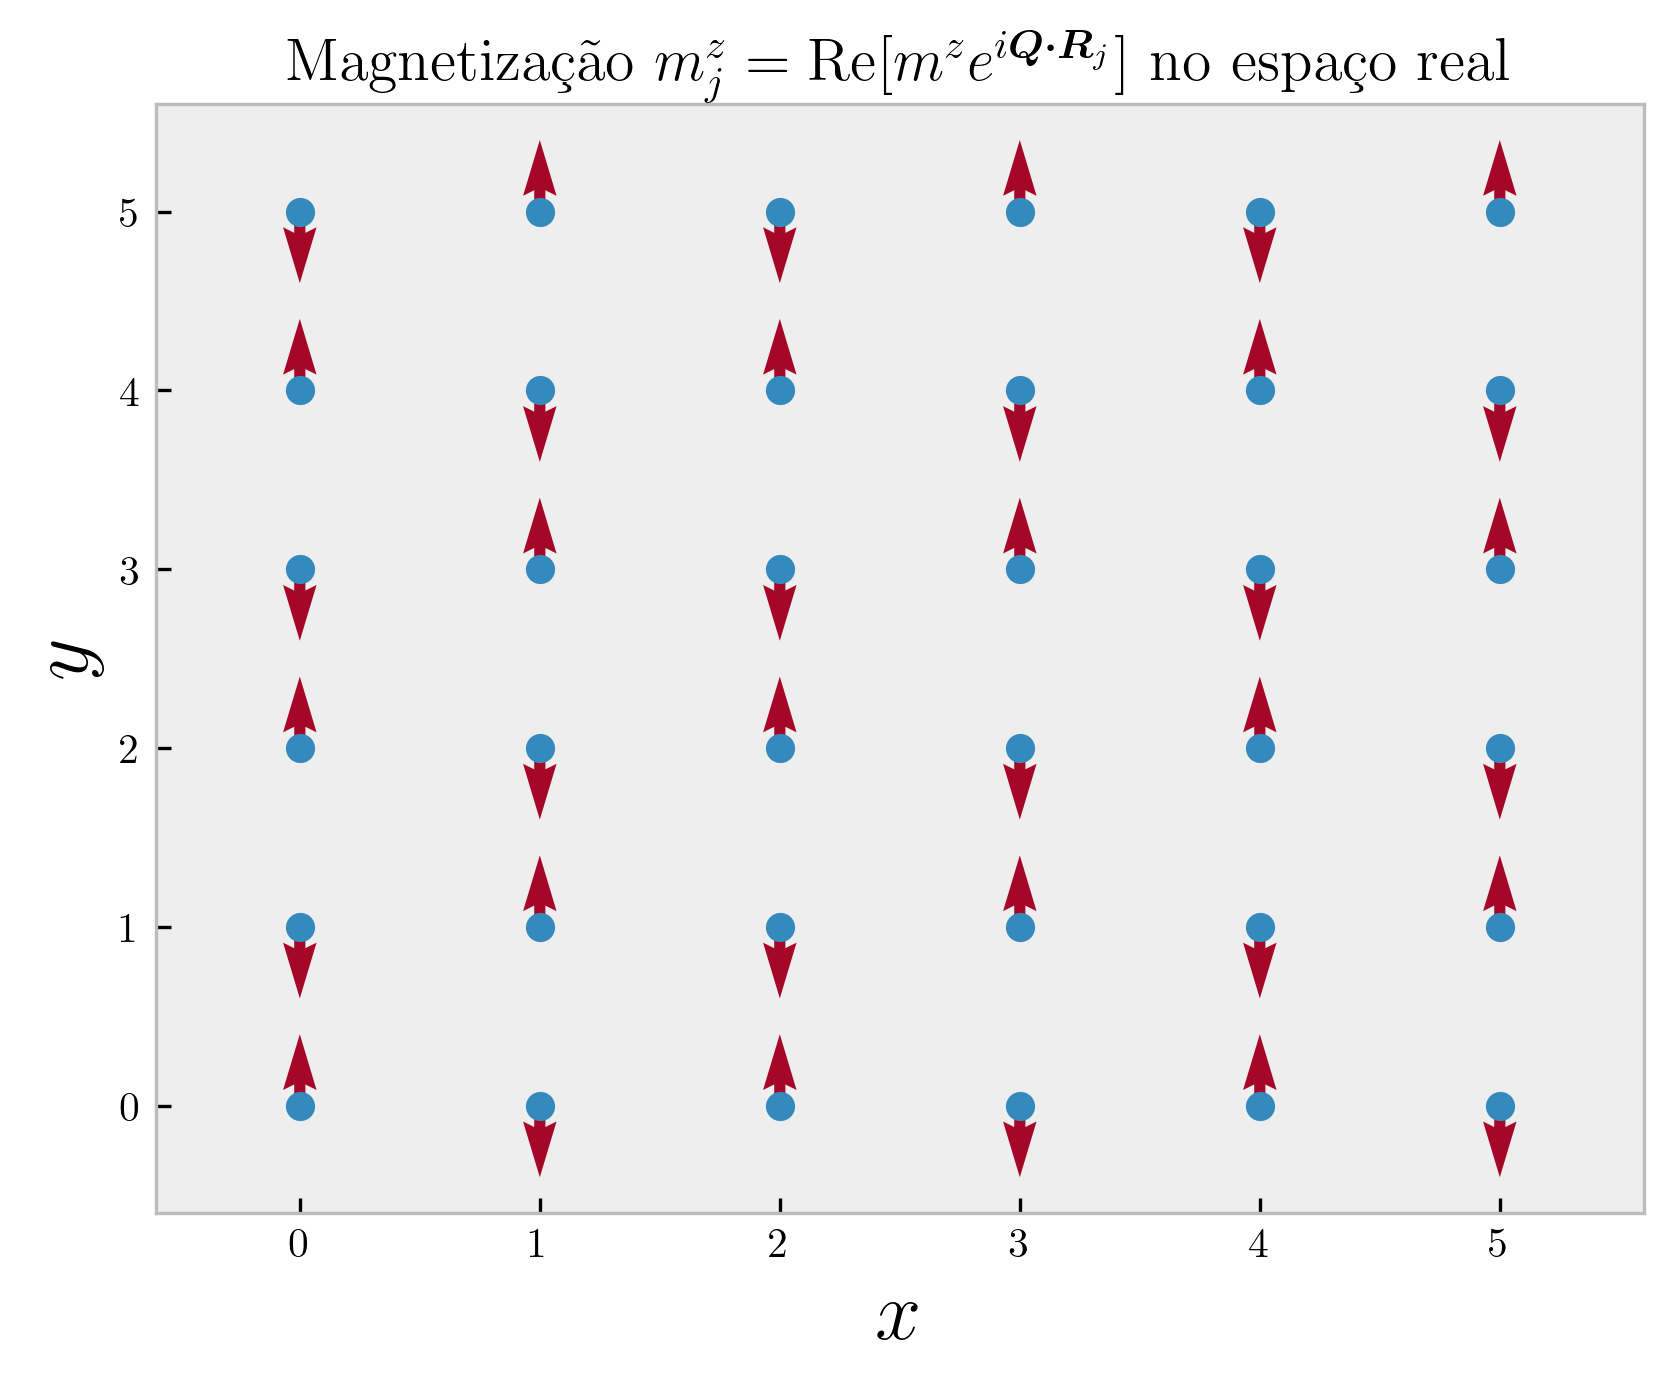
\includegraphics[width=0.75\textwidth]{fig/magnetization-real_space.png}
\caption{Magnetização $m^z_j = \Re[m^z e^{i \bm{Q} \vdot \bm{R}_j}]$ em vermelho para o estado de Néel.}
\label{fig:mag-neel}
\end{figure}

(b) No contexto de campo médio para os operadores de spin $\S_i$, vimos em aula que a hamiltoniana de Hubbard se escreve como
$$
H_{MF} = H_0 - \sum_{i} \bm{m}_i \vdot \S_i + \frac{3}{8U} \sum_{i} \bm{m}_i^2, \quad
\bm{m}_i = \frac{4U}{3} \ev{\S_i},
$$
onde $H_0$ denota a parte não-interagente (\textit{on-site} + \textit{hopping}).

\n

Analisando cada termo por vez:
\begin{itemize}
\item Como sabemos, $H_0$ no espaço de momento $\k$ é dado por $\sum_{\k\s} \eps_{\k} c_{\k\s}^\d c_{\k\s}$. Mas como uma translação $\k \to \k + \bm{Q}$ não afeta a somatória (devido à periodicidade da zona de Brillouin), podemos escrever
$$
H_0 = \frac{1}{2}
\qty{
\sum_{\k\s} \eps_{\k} c_{\k\s}^\d c_{\k\s} +
\sum_{\k\s} \eps_{\k+\bm{Q}} c_{\k+\bm{Q},\s}^\d c_{\k+\bm{Q},\s}
}.
$$

\item O termo $\frac{3}{8U} \sum_{i} \bm{m}_i^2$ resulta simplesmente em $\frac{3}{8U} N m^2$.

\item Utilizando o estado de Néel $\bm{m}_j = \bm{m} \, e^{i \bm{Q} \vdot \bm{R}_j}$, lembre que precisamos tomar a parte real ou, de forma equivalente, somar o hermitiano conjugado e dividir o resultado por 2. Temos que
$$
- \sum_{i} \bm{m}_i \vdot \S_i = -\sum_{i}\sum_{\alpha \beta} c_{i\alpha} \qty(\frac{\bm{\s} \vdot \bm{m}}{2})_{\alpha \beta} c_{i\beta} e^{-i\bm{Q} \vdot \bm{R}_j}.
$$

Tomando as transformadas de Fourier $c_{i\alpha}^\d = \frac{1}{\sqrt{N}} \sum_{\k} e^{-i\k\vdot\R_i}$, temos
$$
= -\frac{1}{N} \sum_{\k,\k'} \sum_{\alpha \beta}
\cancelto{\boxed{N \delta_{\k,\k'+\bm{Q}}}}{\qty{\sum_{i} e^{-i(\k-\k'-\bm{Q})\vdot\R_i}}}
c_{\k\alpha}^\d \qty(\frac{\bm{\s}\vdot\bm{m}}{2})_{\alpha\beta} c_{\k'\beta} =
$$
$$
= - \sum_{\k} \sum_{\alpha \beta}
c_{\k+\bm{Q},\alpha}^\d \qty(\frac{\bm{\s}\vdot\bm{m}}{2})_{\alpha\beta} c_{\k\beta}.
$$


Tomando a parte real ($+ \hc$ e dividindo por 2), o termo $-\sum_{i} \bm{m}_i \vdot \S_i$ resulta em
$$
= - \frac{1}{2} \sum_{\k} \sum_{\alpha\beta}
\qty{
c_{\k+\bm{Q},\alpha}^\d \qty(\frac{\bm{\s}\vdot\bm{m}}{2})_{\alpha\beta} c_{\k\beta}+
c_{\k\alpha}^\d \qty(\frac{\bm{\s}\vdot\bm{m}}{2})_{\alpha\beta} c_{\k+\bm{Q},\beta}.
}
$$
\end{itemize}

Juntando todas as partes de $H_{MF}$, é fácil enxergar que ela se escreve como
$$
H_{MF} = \frac{3}{8U} Nm^2 + \frac{1}{2} \sum_{\k}
\begin{pmatrix}
c_{\k\up}^{\d} & c_{\k\down}^{\d} & c_{\k+\bm{Q},\up}^{\d} & c_{\k+\bm{Q},\down}^{\d}
\end{pmatrix}
\begin{pmatrix}
\eps_{\k} \1 & -\bm{\s} \vdot \bm{m}/2 \\
-\bm{\s} \vdot \bm{m}/2 & \eps_{\k+\bm{Q}} \1
\end{pmatrix}
\begin{pmatrix}
c_{\k\up} \\ c_{\k\down} \\ c_{\k+\bm{Q},\up} \\ c_{\k+\bm{Q},\down}
\end{pmatrix},
$$
onde $\1$ é a matriz identidade $2 \times 2$.

\n

(c) Assumindo uma rede quadrada, onde $\eps_{\k+\bm{Q}}=-\eps_{\k}$, e sem perda de generalidade, que a direção do vetor $\bm{m} = m \vu{z}$ esteja alinhada com eixo $z$, temos que diagonalizar a matriz
$$
M =
\begin{pmatrix}
\eps_{\k} & 0 & -\frac{m}{2} & 0 \\
0 & \eps_{\k} & 0 & \frac{m}{2} \\
-\frac{m}{2} & 0 & -\eps_{\k} & 0 \\
0 & \frac{m}{2} & 0 & -\eps_{\k}
\end{pmatrix}.
$$

Para diagonalizá-la, eu notei que a transformação canônica sugerida na lista está com um pequeno erro. Depois de muitas contas, eu descobri que a transformação correta é
\begin{equation} \label{eq:transf}
\begin{pmatrix}
c_{\k\s} \\ c_{\k+\bm{Q},\s}
\end{pmatrix}
=
\begin{pmatrix}
\cos\theta_{\k} & \s\sin\theta_{\k} \\
-\s\sin\theta_{\k} & \cos\theta_{\k}
\end{pmatrix}
\begin{pmatrix}
\alpha_{\k\s} \\ \beta_{\k\s}
\end{pmatrix},
\end{equation}
$$
T =
\begin{pmatrix}
\cos\theta_{\k} & 0 & \sin\theta_{\k} & 0 \\
0 & \cos\theta_{\k} & 0 & -\sin\theta_{\k} \\
-\sin\theta_{\k} & 0 & \cos\theta_{\k} & 0 \\
0 & \sin\theta_{\k} & 0 & \cos\theta_{\k}
\end{pmatrix},
$$
onde $\s = \pm 1$ para $\up$ ou $\down$ (esse sinal dependente do spin faz toda diferença, sem ele a matriz $M$ não é diagonalizada). Com isso em mente, fazemos as multiplicações de matriz:
$$
T^{\d} M T =
$$
$$
\begin{pmatrix}
\cos\theta_{\k} & 0 & -\sin\theta_{\k} & 0 \\
0 & \cos\theta_{\k} & 0 & \sin\theta_{\k} \\
\sin\theta_{\k} & 0 & \cos\theta_{\k} & 0 \\
0 & -\sin\theta_{\k} & 0 & \cos\theta_{\k}
\end{pmatrix}
\begin{pmatrix}
\eps_{\k} & 0 & -\frac{m}{2} & 0 \\
0 & \eps_{\k} & 0 & \frac{m}{2} \\
-\frac{m}{2} & 0 & -\eps_{\k} & 0 \\
0 & \frac{m}{2} & 0 & -\eps_{\k}
\end{pmatrix}
\begin{pmatrix}
\cos\theta_{\k} & 0 & \sin\theta_{\k} & 0 \\
0 & \cos\theta_{\k} & 0 & -\sin\theta_{\k} \\
-\sin\theta_{\k} & 0 & \cos\theta_{\k} & 0 \\
0 & \sin\theta_{\k} & 0 & \cos\theta_{\k}
\end{pmatrix} =
$$
$$
=
\begin{pmatrix}
\cos\theta_{\k} & 0 & -\sin\theta_{\k} & 0 \\
0 & \cos\theta_{\k} & 0 & \sin\theta_{\k} \\
\sin\theta_{\k} & 0 & \cos\theta_{\k} & 0 \\
0 & -\sin\theta_{\k} & 0 & \cos\theta_{\k}
\end{pmatrix}
\times
$$
$$
\begin{pmatrix}
\eps_{\k}\cos\theta_{\k} + \frac{m}{2}\sin\theta_{\k} & 0 & -\eps_{\k}\cos\theta_{\k}+\frac{m}{2}\sin\theta_{\k} & 0 \\
0 & \eps_{\k}\cos\theta_{\k}+\frac{m}{2}\sin\theta_{\k} & 0 & \eps_{\k}\sin\theta_{\k}-\frac{m}{2}\cos\theta_{\k} \\
-\eps_{\k}\sin\theta_{\k}+\frac{m}{2}\cos\theta_{\k} & 0 & -\eps_{\k}\cos\theta_{\k}-\frac{m}{2}\sin\theta_{\k} & 0 \\
0 & \eps_{\k}\sin\theta_{\k}-\frac{m}{2}\cos\theta_{\k} & 0 & -\eps_{\k}\cos\theta_{\k}-\frac{m}{2}\sin\theta_{\k}
\end{pmatrix} =
$$
$$
\begin{pmatrix}
\eps_{\k}\cos2\theta_{\k} + \frac{m}{2}\sin2\theta_{\k} & 0 & -\eps_{\k}\sin2\theta_{\k}+\frac{m}{2}\cos2\theta_{\k} & 0 \\
0 & \eps_{\k}\cos2\theta_{\k}+\frac{m}{2}\sin2\theta_{\k} & 0 & \eps_{\k}\sin2\theta_{\k}-\frac{m}{2}\cos2\theta_{\k} \\
-\eps_{\k}\sin2\theta_{\k}+\frac{m}{2}\cos2\theta_{\k} & 0 & -\eps_{\k}\cos2\theta_{\k}-\frac{m}{2}\sin2\theta_{\k} & 0 \\
0 & \eps_{\k}\sin2\theta_{\k}-\frac{m}{2}\cos2\theta_{\k} & 0 & -\eps_{\k}\cos2\theta_{\k}-\frac{m}{2}\sin2\theta_{\k}
\end{pmatrix}.
$$

\n

Se $\theta_{\k}$ satisfizer a relação
$$
\eps_{\k} \sin2\theta_{\k} = \frac{m}{2} \cos2\theta_{\k} \iff
\boxed{ \tan2\theta_{\k} = \frac{m}{2\eps_{\k}}, }
$$
a matriz $M$ será diagonalizada:
$$
T^\d M T =
\begin{pmatrix}
\sqrt{\eps_{\k}^2 + m^2/4} & 0 & 0 & 0 \\
0 & \sqrt{\eps_{\k}^2 + m^2/4} & 0 & 0 \\
0 & 0 & -\sqrt{\eps_{\k}^2 + m^2/4} & 0 \\
0 & 0 & 0 & -\sqrt{\eps_{\k}^2 + m^2/4}
\end{pmatrix}.
$$

Obs: é fácil verificar que $\qty{\alpha_{\k\s},\alpha_{\k\s}^\d} = \qty{\beta_{\k\s},\beta_{\k\s}^\d} = 1$ com a transformação \ref{eq:transf}. Não vou explicitar as contas aqui.

\n

(d) Utilizando o índice $p = \pm$ para indexar as energias $E_{\k,p}$, temos que a energia livre de campo médio por sítio é
$$
f = - \frac{1}{\beta N} \ln Z = \frac{3}{8U}m^2 -
\frac{1}{\beta N} \sum_{\k, p, \s} \ln[ 1 + e^{-\beta (E_{\k,p,\s} - \mu)} ].
$$

Usando que $1 + e^{-x} = e^{-x/2} \cdot 2 \cosh x$, o termo da somatória pode ser reescrito como
$$
\frac{1}{\beta N} \sum_{\k, p, \s} \ln[ 1 + e^{-\beta (E_{\k,p} - \mu)} ] =
-\frac{1}{\beta N} \sum_{\k, p, \s} \qty{
-\frac{\beta}{2} (E_{\k,p} - \mu) +
\ln\qty{2 \cosh\qty[\frac{\beta}{2} (E_{k,p} - \mu)] }
} =
$$
$$
=
-\frac{1}{2 N} \sum_{\k, p, \s} \mu -
\frac{1}{\beta N} \sum_{\k, p, \s}
\ln\qty{2 \cosh\qty[\frac{\beta}{2} (E_{k,p} - \mu)] },
$$
onde usei que $\sum_{p} E_{\k,p} = 0$, já que $E_{\k,-} = - E_{\k,+}$. Com isso vemos que $f$ tem a forma
$$
f = f_0 -
\frac{T}{N} \sum_{\k,p,\s}
+ \frac{3}{8U} m^2
\ln\qty{2\cosh\qty[\frac{\beta}{2}(E_{\k,p} - \mu)]} .
$$

(e) Extremizando a energia livre com respeito a $m$ e substituindo $E_{\k,p} = p \sqrt{\eps_{\k}^2 + m^2}$, temos
$$
0 = \pdv{f}{m} =
\frac{3}{4U} m -
\frac{1}{\cancel{\beta} N} \sum_{\k, p, \s}
\frac{\cancel{2}\sinh\qty[\frac{\beta}{2}(E_{\k,p}-\mu)]}{\cancel{2}\cosh\qty[\frac{\beta}{2}(E_{\k,p}-\mu)]} \cdot
\frac{\cancel{\beta}}{2} \, \frac{p m}{\sqrt{\eps_{\k}^2 + m^2}} \implies
$$
$$
\implies \frac{1}{2N} \sum_{\k, p, \s}
\tanh\qty[\frac{\sqrt{\eps_{\k}^2 + m^2} - p\mu}{2T}]
\frac{1}{\sqrt{\eps_{\k}^2 + m^2}} = \frac{3}{4U} .
$$

Tomando $T \to 0$, a tangente hiperbólica tende a $1$. Substituindo $\frac{1}{N} \sum_{\k,p,\s} = \int_{-\infty}^{\infty} \dd{\eps} \rho(\eps)$:
$$
\int_{-\infty}^{\infty} \frac{\rho(\eps)}{\sqrt{\eps^2 + m^2}} \dd{\eps} = \frac{3}{2U}.
$$

A aproximação $\rho(\eps) = (1/4\pi t^2) \ln(t/\abs{\eps})$ é válida para $\abs{\eps} \leq \tau \ll t$ ($\tau$ é um cut-off). Temos então
$$
\frac{3}{2U} = \int_{-\infty}^{\infty} \frac{\rho(\eps)}{\sqrt{\eps^2 + m^2}} \dd{\eps} =
\textcolor{blue}{\int_{-\tau}^{\tau} \frac{\rho(\eps)}{\sqrt{\eps^2 + m^2}} \dd{\eps}} +
\textcolor{red}{\int_{\abs{\eps} \geq \tau} \frac{\rho(\eps)}{\sqrt{\eps^2 + m^2}} \dd{\eps}} =
\textcolor{blue}{I} + \textcolor{red}{J},
$$
onde substituimos a aproximação logarítmica em $I = (1/4\pi t^2) \int_{-\tau}^{\tau} \frac{\ln(t/\abs{\eps})}{\sqrt{\eps^2 + m^2}} \dd{\eps}$ e a integral $0 \leq J < \infty$ tem um resultado finito (não diverge) pois $\rho(\eps)$ é bem comportado para $\abs{\eps} \geq \tau$.

\n

Estudaremos a convergência da integral $I$:
\begin{itemize}
\item Para $m > 0$, provarei que $I < \infty$ converge. Temos que $\frac{1}{\sqrt{\eps^2+m^2}} \leq \frac{1}{m}$. Assim:
$$
I \leq \frac{1}{4\pi t^2 m} \int_{-\tau}^{\tau} \Big( \ln t - \ln\abs{\eps} \Big) \dd{\eps} =
\frac{1}{4\pi t^2 m} \Big[ 2\tau \ln t - 2 \int_{0}^{\tau} \ln\eps \dd{\eps} \Big] .
$$

Lembrando que $\int \ln x \dd{x} = x \ln x - x$ e que $\displaystyle{\lim_{x\to 0} (x \ln x) = 0}$, obtemos que a integral $I$ converge para todo $m > 0$:
$$
I \leq \frac{\tau}{2\pi t^2 m} \qty[1 + \ln(\frac{t}{\tau})] < \infty.
$$

Isso mostra que, dado $m > 0$, a interação correspondente $U = \frac{3}{2(I+J)} > 0$ é maior que zero (ela seria zero caso $I + J = \infty$).

\item Para $m = 0$ provarei que $I = \infty$ diverge. Nesse caso, substituindo a variável $x = t/\eps$ temos
$$
I = \frac{1}{2\pi t^2} \int_{0}^{\tau} \frac{\ln(\frac{t}{\eps})}{\eps} \dd{\eps} =
\frac{1}{2\pi t^2}
\int_{t/\tau}^{\infty} \frac{\ln x}{x} \dd{x} =
\frac{1}{2\pi t^2} \cdot \eval{\frac{(\ln x)^2}{2}}_{t/\tau}^{\infty} = \infty.
$$

Portanto $I = \infty$ diverge e, consequentemente, para $m = 0$ o $U$ correspondente é zero.
\end{itemize}

Esses dois itens demonstram que $U_c = 0^+$.

A solução obtida corresponde a um isolante pois vemos que o módulo da magnetização $m$ se comporta como um gap na relação de dispersão $E_{\k,\pm} = \pm \sqrt{\eps_{\k}^2 + m^2/4}$ e, para $n_e = 1$, a banda de baixo é toda preenchida, de maneira que conseguimos interpretar o resultado como um isolante de bandas, onde o gap é originado pelo estabilidade da fase antiferromagnética.

O resultado obtido mostra que, para qualquer interação $U > 0$, temos uma solução $m > 0$ estável que extremiza a energia livre. Isso mostra a estabilidade do estado antiferromagnético. Lembrando do que estudamos para isolantes de Mott onde $U/t \geq 1$, temos que o material correlacionados é um isolante (de Mott) e a fase antiferromagnética também é estável.

\textbf{AS IDEIAS ESTÃO ACIMA. ORGANIZAR O TEXTO.}



\pagebreak

\section{Modelo de Heisenberg na rede triangular}

Para a rede triangular com vetores unitários $\vb{a}_1 = (1,0)$ e $\vb{a}_2 = \qty(\frac{1}{2}, \frac{\sqrt{3}}{2})$ e os vetores correspondentes no espaço recíproco são $\vb{b}_1 = \frac{4\pi}{\sqrt{3}} \qty(\frac{\sqrt{3}}{2}, -\frac{1}{2})$ e $\vb{b}_2 = \frac{4\pi}{\sqrt{3}} \qty(0, 1)$. Temos que todos os possíveis vetores $\bm{\delta}$ são $\pm\vb{a}_1, \pm\vb{a}_2$ e $\pm (\vb{a}_2 - \vb{a}_1)$. Portanto
$$
J(\q) = \frac{J}{2} \sum_{\bm{\delta}} e^{-i \q \vdot \bm{\delta}} =
J \qty{\cos(\q \vdot \vb{a}_1) + \cos(\q \vdot \vb{a}_2) + \cos[\q \vdot (\vb{a}_2 - \vb{a}_1)]} =
$$
$$
= J \qty[\cos(q_x) + \cos(\frac{q_x}{2} + \frac{\sqrt{3} q_y}{2}) + \cos(\frac{q_x}{2} - \frac{\sqrt{3} q_y}{2})].
$$

Usando que $\cos(x+y) + \cos(x-y) = 2 \cos(x) \cos(y)$, temos que
$$
J(\q) = J \qty[\cos(q_x) + 2 \cos(\frac{q_x}{2}) \cos(\frac{\sqrt{3} q_y}{2})].
$$

Tomando o gradiente e igualando a zero temos
$$
\pdv{J}{q_x} = J \qty[-\sin(q_x) - \sin(\frac{q_x}{2}) \cos(\frac{\sqrt{3} q_y}{2})] = 0,
$$
$$
\pdv{J}{q_y} = - \sqrt{3} J \cos(\frac{q_x}{2}) \sin(\frac{\sqrt{3} q_y}{2}) = 0.
$$

Escolhendo $\sin(\frac{\sqrt{3} q_y}{2}) = 0$, podemos tomar $q_y = \frac{2\pi}{\sqrt{3}}$, de maneira que $\cos(\frac{\sqrt{3} q_y}{2}) = -1$ e, portanto, $\sin(q_x) - \sin(q_x/2) = 2 \cos(\frac{3 q_x}{4}) \sin(\frac{q_x}{4}) = 0$. Escolhendo $\cos(\frac{3q_x}{4}) = 0$, tomamos $q_x = \frac{2\pi}{3}$. Essas escolhas nos dão $\vb{Q} = \qty(\frac{2\pi}{3}, \frac{2\pi}{\sqrt{3}}) \in \text{BZ}$ e $J(\vb{Q}) = -\frac{3}{2} J = \displaystyle{\min_{\q} J(\q)}$. Assim, a energia do estado fundamental é $E_0 / N  = -\frac{3}{2} S^2$, que é o resultado esperado para todos os spins formando um ângulo de $120^\circ$.

Fazendo o esboço da magnetização $m_j = m e^{i \vb{Q} \vdot \vb{R}_j}$ no espaço real, obtemos a Figura \ref{fig:mag-triang}:
\begin{figure}[H]
\centering
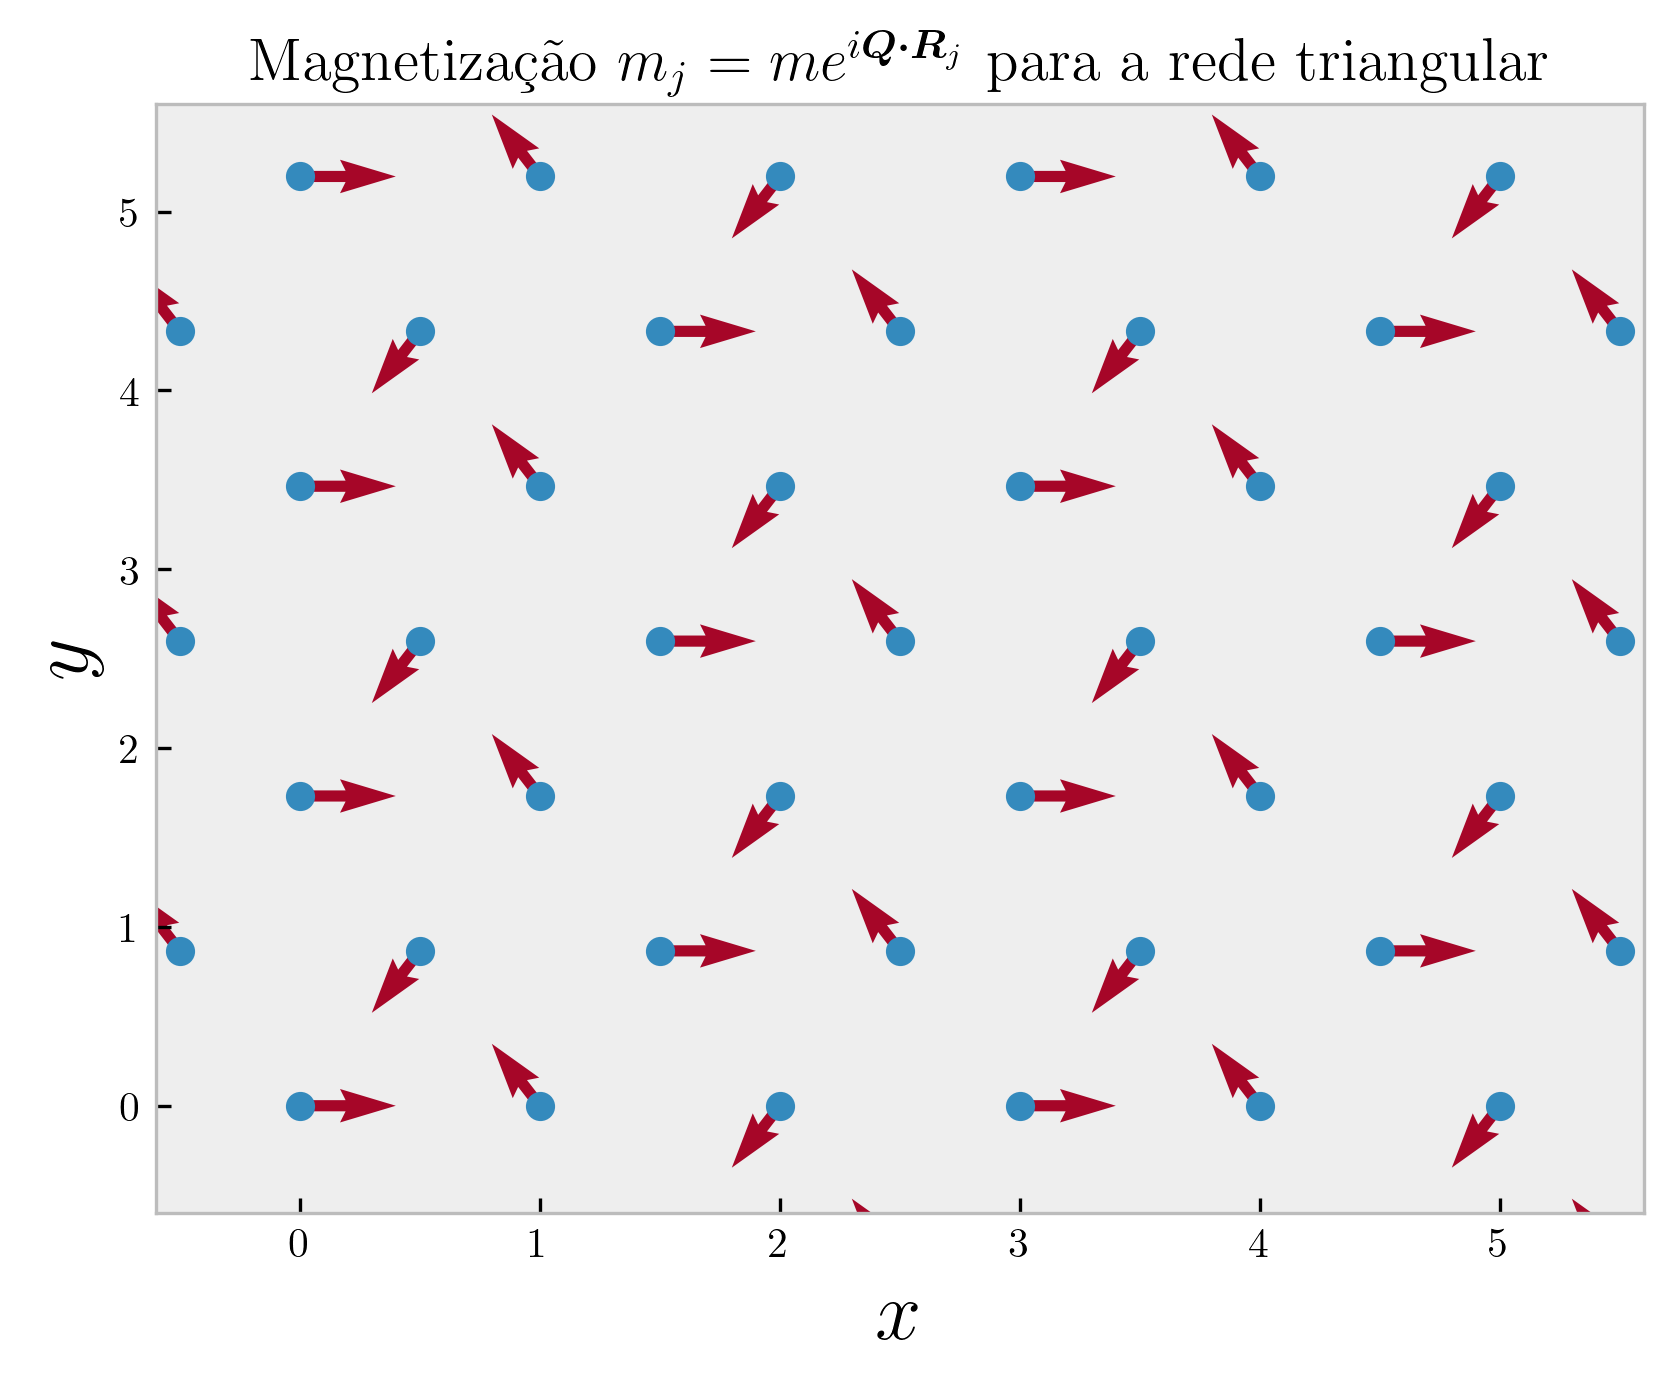
\includegraphics[width=0.75\textwidth]{fig/mag_triang-real_space.png}
\caption{Magnetização $m^z_j = \Re[m^z e^{i \bm{Q} \vdot \bm{R}_j}]$ em vermelho para a rede triangular.}
\label{fig:mag-triang}
\end{figure}

\pagebreak

\section{Transformação de Bogoliubov bosônica}

(a) Invertendo $T$ temos que
$$
\begin{pmatrix}
\alpha_{\k} \\ \alpha_{-\k}^\d
\end{pmatrix}
=
T^{-1}
\begin{pmatrix}
a_{\k} \\ a_{-\k}^\d
\end{pmatrix}
=
\begin{pmatrix}
\cosh\theta_{\k} & \sinh\theta_{\k} \\
\sinh\theta_{\k} & \cosh\theta_{\k}
\end{pmatrix}
\begin{pmatrix}
a_{\k} \\ a_{-\k}^\d
\end{pmatrix}
$$

Portanto
$$
[\alpha_{\k}, \alpha_{-\k}] =
\cosh\theta_{\k}\sinh\theta_{\k} \cancelto{0}{[a_{\k}, a_{-\k}]} +
\cosh^2\theta_{\k} \cancelto{1}{[a_{\k}, a_{\k}^\d]} +
\sinh^2\theta_{\k} \cancelto{-1}{[a_{-\k}^\d, a_{-\k}]} +
\cosh\theta_{\k}\sinh\theta_{\k} \cancelto{0}{[a_{-\k}^\d, a_{\k}^\d]} +
$$
$$
= \cosh^2\theta_{\k} - \sinh^2\theta_{\k} = 1.
$$

\n

(b) Temos que
$$
T^\d M T =
\begin{pmatrix}
\cosh\theta_{\k} & -\sinh\theta_{\k} \\
-\sinh\theta_{\k} & \cosh\theta_{\k}
\end{pmatrix}
\begin{pmatrix}
1 & \gamma_{\k} \\
\gamma_{\k} & 1
\end{pmatrix}
\begin{pmatrix}
\cosh\theta_{\k} & -\sinh\theta_{\k} \\
-\sinh\theta_{\k} & \cosh\theta_{\k}
\end{pmatrix}
=
$$
$$
=
\begin{pmatrix}
\cosh(2\theta_{\k}) - \gamma_{\k}\sinh(2\theta_{\k}) & \gamma_{\k}\cosh(2\theta_{\k}) - \sinh(2\theta_{\k}) \\
\gamma_{\k}\cosh(2\theta_{\k}) - \sinh(2\theta_{\k}) & \cosh(2\theta_{\k}) - \gamma_{\k}\sinh(2\theta_{\k})
\end{pmatrix}.
$$

Vemos então que, para a matriz acima ser diagonal, tem-se que $\tanh(2\theta_{\k}) = \gamma_{\k}$. Substituindo isso obtemos
$$
T^\d M T =
\frac{1}{2}
\begin{pmatrix}
2\sqrt{1-\gamma_{\k}^2} & 0 \\
0 & 2\sqrt{1-\gamma_{\k}^2}
\end{pmatrix},
$$
onde identificamos $\omega_{\k} = 2\sqrt{1-\gamma_{\k}^2}$.

Com a transformação de Bogoliubov e as relações de comutação deduzidas é fácil ver que a hamiltoniana transformada se escreve como
$$
H_{SW} = \frac{1}{2} \sum_{\k} \qty(\omega_{\k} \alpha_{\k}^\d \alpha_{\k} + \omega_{\k}).
$$


\pagebreak

\section{Ondas de spin}

(a)



\end{document}
